\section{Routing}

Das Routing in einer Ruby on Rails Applikation wird in der Konfigurationsdatei \emph{config/routes.rb} definiert.
Da alle Ressourcen in dieser Applikation relativ RESTful sind, wurden grösstenteils die \emph{resource} Routing-Helper verwendet.
Diese generieren, dem Rails-Standard \cite{default_controller_actions} entsprechend, alle notwendigen Routes, um CRUD Operationen auszuführen.

Diese können auch genested werden, um so die dahinterliegende Datenstruktur besser zu veranschaulichen. So hat beispielsweise
ein Assessment mehrere Tasks und mit einem \emph{POST /assessments/:id/tasks} kann eine neue Aufgabe erstellt und direkt dem entsprechenden Assessment
zugeordnet werden. Im \emph{member} Block werden ausserdem die zusätzlichen Routes definiert, die für das starten, stoppen und Auswerten des Assessments
benötigt werden.

\begin{codebox}
\begin{minted}{ruby}
resources :assessments do
  resources :tasks, except: :index
  resources :invitations, only: %i[new create]

  member do
    patch :start
    patch :close
    get :summary
  end
end
\end{minted}
\end{codebox}

Dabei wurden nicht alle Ressourcen ineinander genested, da die Pfade sonst unübersichtlich lang werden.
Dennoch sollten diese bezogen auf die Datenstruktur und das UI-Design sinnvoll miteinander verknüpft sein. Mit der \mintinline{ruby}{shallow: true}
Option werden die folgenden Pfade \enquote{flattened}.

\begin{codebox}
\begin{minted}{ruby}
resources :tasks, only: [], shallow: true do
  resources :solutions, except: %i[index destroy] do
    resources :comments, only: :create
  end
end
\end{minted}
\end{codebox}

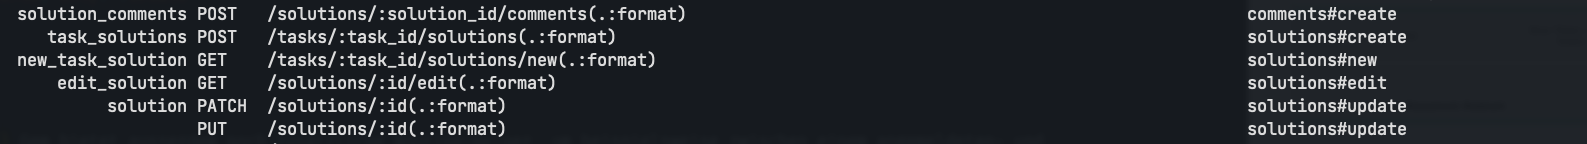
\includegraphics[width=\textwidth]{images/routes.png}

Für einen eingeloggten Benutzer ändert sich ausserdem der Root-Pfad (\emph{/}) vom login-screen zu der Assessment-Übersichtsseite.
Dies wurde anhand der Devise Helpern konfiguriert.

\begin{codebox}
\begin{minted}{ruby}
authenticated do
  root 'assessments#index', as: :authenticated_root
end

devise_scope :user do
  root 'devise/sessions#new'
end
\end{minted}
\end{codebox}
